%--------------------------------------------------------------
% tesi.tex 
%--------------------------------------------------------------
% Corso di Laurea in Informatica 
% http://if.dsi.unifi.it/
% @Facolt\`a di Scienze Matematiche, Fisiche e Naturali
% @Universit\`a degli Studi di Firenze
%--------------------------------------------------------------
% - template for the main file of Informatica@Unifi Thesis 
% - based on Classic Thesis Style Copyright (C) 2008 
%   Andr\'e Miede http://www.miede.de   
%--------------------------------------------------------------

\documentclass[twoside,openright,titlepage,fleqn,
,	headinclude,12pt,a4paper,BCOR5mm,footinclude,table]{scrbook}
%--------------------------------------------------------------
\newcommand{\myItalianTitle}{Titolo In Italiano\xspace}
\newcommand{\myEnglishTitle}{Title In English\xspace}
% use the right myDegree option
\newcommand{\myDegree}{Corso di Laurea in Informatica\xspace}
%\newcommand{\myDegree}{
	%Corso di Laurea Specialistica in Scienze e Tecnologie 
	%dell'Informazione\xspace}
\newcommand{\myName}{Terrosi Francesco\xspace}
\newcommand{\myProf}{Bondavalli Andrea\xspace}
\newcommand{\myOtherProf}{Strigini Lorenzo\xspace}
\newcommand{\myFaculty}{
	Scuola di Scienze Matematiche, Fisiche e Naturali\xspace}
\newcommand{\myUni}{\protect{
	Universit\`a degli Studi di Firenze}\xspace}
\newcommand{\myLocation}{Firenze\xspace}
\newcommand{\myTime}{Anno Accademico 2018-2019\xspace}
\newcommand{\myVersion}{Version 0.1\xspace}
%--------------------------------------------------------------

\usepackage[italian]{babel}
\usepackage[latin1]{inputenc} 
\usepackage[T1]{fontenc} 
\usepackage[square,numbers]{natbib} 
\usepackage[fleqn]{amsmath}  
\usepackage{ellipsis}
\usepackage{listings}
\usepackage{subfig}
\usepackage{caption}
\usepackage{appendix}
\usepackage{siunitx}
\usepackage{url}

%--------------------------------------------------------------
\usepackage{dia-classicthesis-ldpkg}
%--------------------------------------------------------------


%
% Options for classicthesis.sty:
% tocaligned eulerchapternumbers drafting linedheaders 
% listsseparated subfig nochapters beramono eulermath parts 
% minionpro pdfspacing
\usepackage[eulerchapternumbers,linedheaders,subfig,beramono,eulermath,
parts]{classicthesis}
%--------------------------------------------------------------
\newlength{\abcd} % for ab..z string length calculation
% how all the floats will be aligned
\newcommand{\myfloatalign}{\centering} 
\setlength{\extrarowheight}{3pt} % increase table row height
\captionsetup{format=hang,font=small}
%--------------------------------------------------------------
% Layout setting
%--------------------------------------------------------------
\usepackage{geometry}
\geometry{
	a4paper,
	ignoremp,
	bindingoffset = 1cm, 
	textwidth     = 13.5cm,
	textheight    = 21.5cm,
	lmargin       = 3.5cm, % left margin
	tmargin       = 4cm    % top margin 
}




%%
%% Julia definition (c) 2014 Jubobs
%%
\lstdefinelanguage{Julia}%
  {morekeywords={abstract,break,case,catch,const,continue,do,else,elseif,%
      end,export,false,for,function,immutable,import,importall,if,in,%
      macro,module,otherwise,quote,return,switch,true,try,type,typealias,%
      using,while},%
   sensitive=true,%
   alsoother={},%
   morecomment=[l]\#,%
   morecomment=[n]{\#=}{=\#},%
   morestring=[s]{"}{"},%
   morestring=[m]{'}{'},%
}[keywords,comments,strings]%

\lstset{%
    language         = Julia,
    basicstyle       = \ttfamily,
    keywordstyle     = \bfseries\color{blue},
    stringstyle      = \color{magenta},
    commentstyle     = \color{ForestGreen},
    showstringspaces = false,
}
%%%

\usepackage{tikz}
\usetikzlibrary{arrows}
\usetikzlibrary{positioning}
\tikzset{main node/.style={circle,fill=blue!20,draw,minimum size=1cm,inner sep=0pt},
            }



%--------------------------------------------------------------
\begin{document}
\frenchspacing
\raggedbottom
\pagenumbering{roman}
\pagestyle{plain}
%--------------------------------------------------------------
% Frontmatter
%--------------------------------------------------------------


%--------------------------------------------------------------
% titlepage.tex (use thesis.tex as main file)
%--------------------------------------------------------------
\begin{titlepage}
	\begin{center}
   	\large
      \hfill
      \vfill
      \begingroup
         \includegraphics[scale=0.15]{logo/LOGO}\\
%			\spacedallcaps{\myUni} \\ 
			\myFaculty \\
			\myDegree \\ 
			\vspace{0.5cm}
         \vspace{0.5cm}    
           
      \endgroup 
      \vfill 
      \begingroup
      	\color{Maroon}\spacedallcaps{\myItalianTitle} \\ $\ $\\
	\bigskip
      \endgroup
      \spacedlowsmallcaps{\myName} \\ $\ $\\
      \spacedlowsmallcaps{\myProf} \\ $\ $
      \spacedlowsmallcaps{\myOtherProf}
      \vfill 
      \vfill
    
      \vfill
      \vfill
      \myTime
      \vfill                      
	\end{center}        
\end{titlepage}   
%--------------------------------------------------------------
% back titlepage
%--------------------------------------------------------------
   \newpage
	\thispagestyle{empty}
	\hfill
	\vfill
	\noindent\myName: 
	\textit{\myItalianTitle,} 
	\myDegree, \textcopyright\ \myTime
%--------------------------------------------------------------
% back titlepage end
%--------------------------------------------------------------

\pagestyle{scrheadings}
%--------------------------------------------------------------
% Mainmatter
%--------------------------------------------------------------
\pagenumbering{arabic}
% use \cleardoublepage here to avoid problems with pdfbookmark
%\include{intro} % use \myChapter command instead of \chapter
%\cleardoublepage\myPart{Part I}
%\include{chapter01}
%\cleardoublepage\myPart{Part II}
%\include{chapter02}
%\include{chapter03}

\paragraph{Abstract}\mbox{}\\*\\*

Abstract

\tableofcontents
\listoftables
\listoffigures
\chapter{Introduzione}

Sistemi informatici ormai ovunque (Cosa sono, esempi)

\section{Cyber-physical systems of systems}

\begin{itemize}
	\item Cosa sono i sistemi cyber-fisici
	\item safety e dependability
	\item safety-assessment classicamente?
\end{itemize}

\chapter{Automotive - State of art}

Self driving cars are one of the hottest topics of the decade. Artificial Intelligences specifically trained to drive with machine learning techniques demonstrated that it's possible for a computer to drive cars. However, a failure of these systems may have very serious consequences that could result in people being injuried, or killed. At the same time, it is a problem to certify the ultra-high dependability requirements demanded. In this chapter, today's problems regarding the safety issues related to self driving cars are reviewed, for that it was decided to conduct this study.

\section{Autonomous Cars as CPS}

In order for a car to be able to drive by itself, suitable hardware and software are required. This makes autonomous cars cyber physical systems, and the possible catastrophic consequences that a failure in/of these systems can cause, make them fall under the set of critical systems.

To sense and map the surrounding environment, the system collects data from multiple sensors. Some of the most important sensors and their purposes are listed here:

\begin{itemize}
	\item GPS
	\begin{itemize}
		\item[$\rightarrow$] High precision GPS sensors are used to estimate the exact position on the vehicle in the world
	\end{itemize}
	\item Odometry \& IMU sensors
	\begin{itemize}
		\item[$\rightarrow$] These sensors are worth for detecting changes in the position of the car and of the objects in the environment over time
	\end{itemize}
	\item Cameras
	\begin{itemize}
		\item[$\rightarrow$] Cameras are literally the \textsl{eyes} of the system. Images captured are usually processed with image recognition software
	\end{itemize}
	\item Lidars \& Radars
	\begin{itemize}
		\item[$\rightarrow$] Lidars can be seen as the evolution of conventional radars. Data combined from these sensors serve the purpose of mapping the environment and detect obstacles and objects around the car
	\end{itemize}
\end{itemize}

Outputs from these sensors are combined and given to the car's control system.
An abstraction of the software architecture is shown in this figure:
\begin{figure}[h!]
	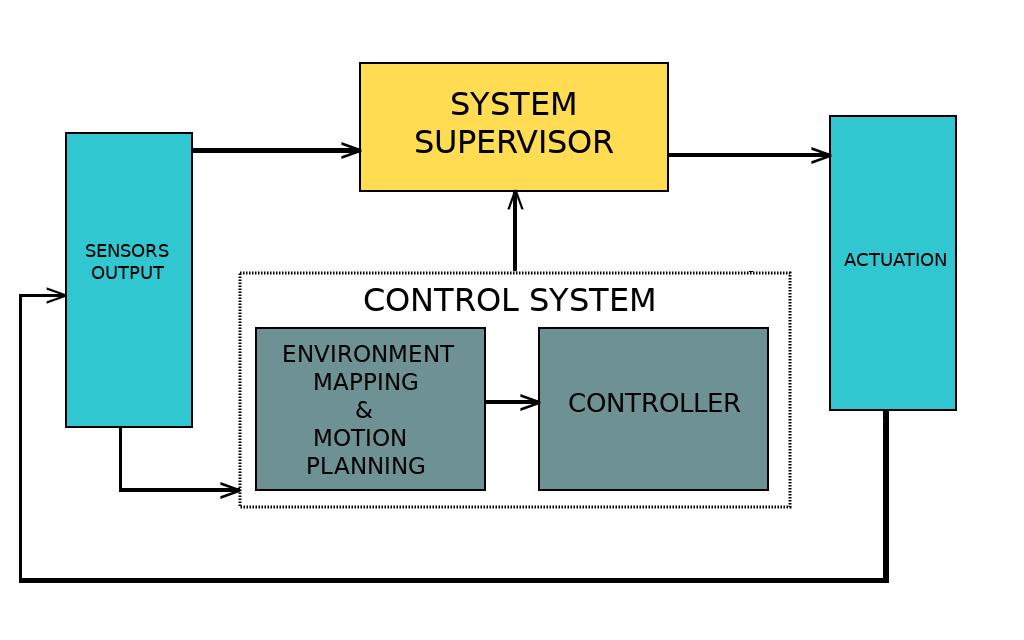
\includegraphics[width=\textwidth]{img/av-architecture.png}
	\caption{High-level abstraction of the system's software architecture}
\end{figure}

Data from sensors are inputs of the control system, here simplified as composed by two constituent systems: one in charge of collecting data directly from the sensors, process them in order to build an \textsl{occupancy grid}\footnote{A matrix mapping the environment, the cells $a_{i,j}$ are flagged with 0 if there's no object at coordinates $i,j$, 1 if occupied.} to map the surrounding area and to create a physical model of the environment in order to follow the correct route to the destination without crashing. The Controller (usually composed as a combination of a Velocity Controller\footnote{Controller in charge of adjusting the vehicle's speed} and a Steering Controller\footnote{Controller that determines the steering angle}) uses these data to adjust the values on the actuators controlling the movements of the car: throttle, brake and steer.\newline
Due to the criticity of their task, it's mandatory to have a System Supervisor, a System in charge of detecting possible hardware failures or wrong outputs\footnote{With \textsl{"wrong"} is intended not only outputs out of the domain space but also outputs that would cause the system to fail (e.g. causing a crash)} from the Control System and, if needed, activate a corrective routine.

The System Supervisor is the main failure avoidance component of such systems. Of course there may be specific checks when data are processed, but the last decision is up to this system's monitor and the underestimation of its importance can lead to dramatic consequences, such as the 2018 accident in Arizona, where a woman was killed by a self-driving car during a test run.\cite{arizuber} Further inspections showed that the car's radar and LiDAR sensors detected the victim almost 6 seconds before the impact and it took 4 seconds circa to infer that there was an obstacle on the road and that an emergency brake was needed. However, this safety-checker was disabled during tests for "smoother rides", causing the accident.\cite{govarizuber}\newline\newline
The extreme complexity of these systems raise concerns among the experts: the need to find a new point of view to study and test the safety of these systems, and the need to sensitise about safety culture.\cite{koopman}


\section{Safety And Autonomous Vehicles}

According to a SAE International tentative to classify self-driving cars' autonomy, the level of automation can be divided in 6 tiers, ranging from 0 to 5. Level 0 means no autonomy: a human driver just drives the car; level 5 means that there's no need of human intervention at all and the car is not only capable of driving safely on the road, but it must be able to avoid catastrophic failures that may seriously harm (or kill) people.
The more autonomous the car is, the higher the dependability requirements are for it to be put on public roads.
It is a well known issue that demonstrating a system's dependability is not an easy task for itself, it gets even harder with ultra-high dependability systems such as these are. In adition to the problem itself, demonstrating autonomous cars' dependability has two more problems to deal with: how to safely and effectively test the system and the presence of neural networks, for which it's very hard to understand why it returned the output $y$, given the input $x$.

Lots of studies demonstrated that it's unthinkable to just test cars on the roads. One of these, that we will refer to as the RAND Study, answers the question of how many miles of driving would it take to demonstrate autonomous vehicles' reliability using classical statistical inference, saying that if autonomous cars fatality rate was 20\% lower than humans', it would take more than 500 years with \textsl{"a fleet of 100 autonomous vehicles being test-driven 24 hours a day, 365 days a year at an average speed of 25 miles per hour"}.\cite{randstudy}\newline
The validation of ultra-high dependability requirements for safety-critical systems is a well known problem in safety literature and has not been introduced by the advent of autonomous cars. In fact, the RAND study is nothing but a specific case of the problem considered in a work published in 1993 by Littlewood \& Strigini, in which the same concepts are discussed and generalized for every ultra-high dependability system.\cite{littlewoodStrigini}\newline
The main problem with the RAND study approach is that future failures frequency can not be predicted just using the observed one. Not just for the quantitative results of the impossibility of it, but also because this approach can not work: an observed frequency failure of $0$ would lead to optimistic (and probably harmful) predictions. Luckily, this problem is surmountable, as shown in \textsl{this}\cite{zhaoStrigini} work by Zhao et al.\newline

Validating the dependability requirements of an autonomous car seems a hard task already. Things are made even harder by the fact that these cars are driven by neural networks.\newline
In these years there is a huge growing interest in the \textsl{machine learning} sector, and this has made that a lot of progress was done in the research. It's also thanks to these progresses that autonomous cars now seem like something we can achieve, since these AIs gave surprising results with their skills, and big brands such as \textsl{Uber} and \textsl{Tesla} are putting more and more efforts in AI research.
This new wave of AI research is deeply changing the way we interact with computer systems, and surprising results were achieved with neural networks.\newline
These tools have proven to outclass \textsl{"classic"} software solutions (intended as non-neural network) in a lot of tasks, ranging from \textsl{Object Detection}\cite{retinaNet} to \textsl{Gaming}\cite{alphaGo} problems, performing even better than humans.\cite{alphaGoBeatsMan}
The complexity of the environment in which the system performs and the need of quick decision-making procedures and fast responses to events that \textsl{cannot} be planned with \textsl{"classic"} software, make neural networks the perfect tool to achieve the task of a car being able to drive by itself, thanks to their ability to handle multiple situations that were not explicitly written in the software. However, this raises serious issues about the safety of the whole system for many reasons.\newline

If neural networks gave promising results on one hand, and they seem the only way to achieve goals such as autonomous cars, on the other hand it has been shown many times how weird a network's prediction can get when \textsl{minimally} perturbating the inputs\cite{stupidnn} and how high the confidence interval can be.\cite{foolnn} The lack of official regulations and certifications for this kind of software, as well as the need to truly understand neural networks, is raising concerns on how dependable these systems can be and consciousness is now growing on the topic, asking for more regulations on companies developing advanced AIs.\cite{elonmusk}\newline

\section{Controller - Checker Problem}


The interaction between the Control System and the System Supervisor is at the core of the car's movements. The Control System, or \textsl{Primary Component}, is the software performing the main computations of the system, required to drive the car. In a context like this, it's mandatory to have fault-tolerance mechanisms such as the System Supervisor, to avoid catastrophic failures. This kind of architecture is a must for these systems, due to the extremely high dependability requirements they have, in order to try to cover all the possible failures that may happen. The state space of such systems may be sketched as in figure 7.

\begin{figure}[h!]
	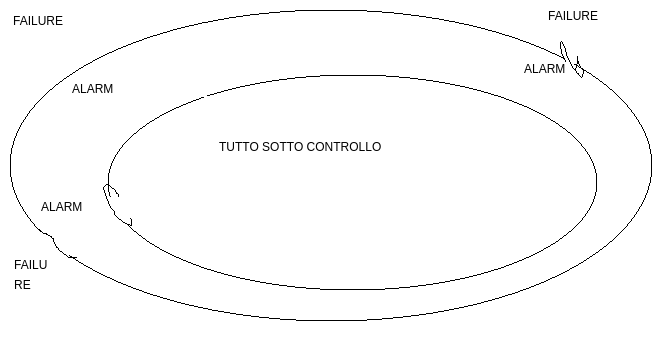
\includegraphics[width=\textwidth]{img/state-space.png}
	\caption{Sketch of the system's safe states}
\end{figure}

We consider \textsl{safe states} all the states in which the Control System produces an output that would not result in a crash.

Imagine that an autonomous car is riding when suddenly an obstacle appears. If the Primary correctly detects the obstacles it should aoutonomously apply a safety-measure to \textbf{avoid} a transition in an \textsl{alert state}. If the controller doesn't see the obstacle, \textsl{or} detects it but keeps throttling, there is a transition from a \textsl{safe-state} to an \textsl{alert-state}, in which the failure-avoidance components turn in. The System Supervisor's duty is now to launch a corrective-routine that will put the system in a fail-safe state (e.g. by applying the safety-brake and turning off the engine). An error of the Supervisor will inevitably cause the system to fail, as a result of the failure of both components, leading in a failure state (the crash happened). If we model the system's failures in this way, the level of safety of the system can be represented as the union of the failure area covered by the Controller and the one covered by the Supervisor

This problem is nothing but a generalization (related to safety) of the asymmetric fault-tolerant architecture for computer systems: the idea of having a \textsl{Primary Component} that performs the main computations, and a \textsl{Primary Checker} in charge of detecting (and correcting) possible errors of the Primary.\newline
The problem of assessing the dependability of these simpler (but still complex) systems is a well known topic in literature and was explored in different studies. In a relatively recent work published by \textsl{Popov} and \textsl{Strigini} in 2010, it is shown that the probability of a system failing on a specific input (or set of inputs), strictly depends on both the coverage of the Primary \textsl{and} the Primary Checker, as shown in the figure above.\cite{striginiPopov}

In the context of self-driving cars we want the area covered by the primary to be the largest possible. This is done by intensive training of the neural networks that will control the car. As long as the network is trained \textsl{"properly"}, the control system should be able to handle most of the dangerous situations that may happen. At one point, it is possible that the Controller learns to handle the \textsl{"alert states"} covered by the System Supervisor, reducing the overall contribution to the system's safety given by the latter.

Another possibility is that during the training, a portion of the failure area covered by the controlller becomes uncovered. This could result in a situation in which some of the previously safe states are now alarm state, representing a serious harm to the system's dependability. Since the coverage area provided by the System Supervisor can not change without changing its implementation (it doesn't "learn" automatically), a transition to one of these states would now inevitably result in a failure.

All these considerations and the lack of literature on the topic for these new systems such as autonomous cars, lead us to begin a study on the emergent behaviour resulting from the interaction of a neural network control system and a \textsl{"classic"} error checker, on what happens when the network is \textsl{taught} by a supervisor during the training and how performance metrics of these 2 components can be computed.\newline

In the next sections we present and discuss the development and implementation of an experimental methodology to study these aspects.

\begin{minipage}[c]{\textwidth}
	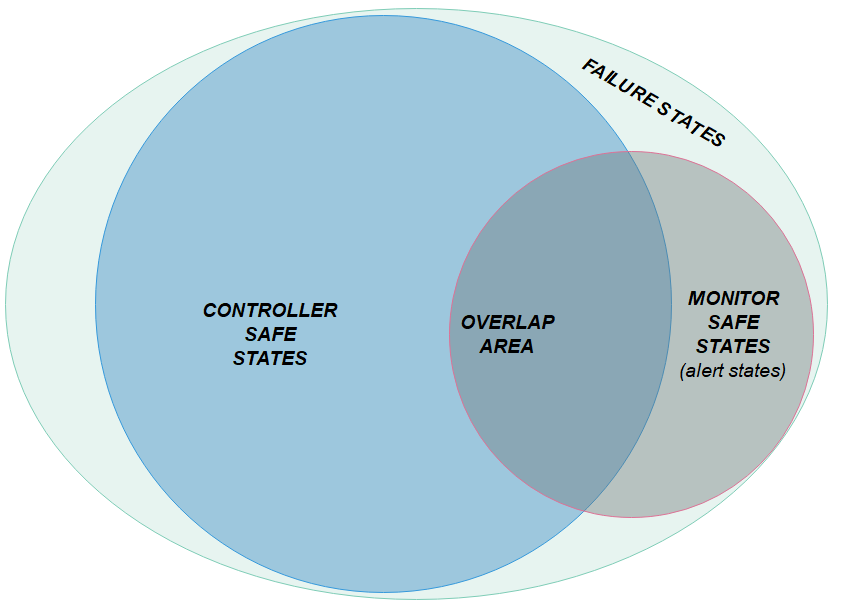
\includegraphics[width=\textwidth]{img/area-growth-good.png}
	\captionof{figure}{The states covered by the Controller are now the ones previously covered, plus some states previously covered just by the Monitor}
	\vspace{0.5cm}
	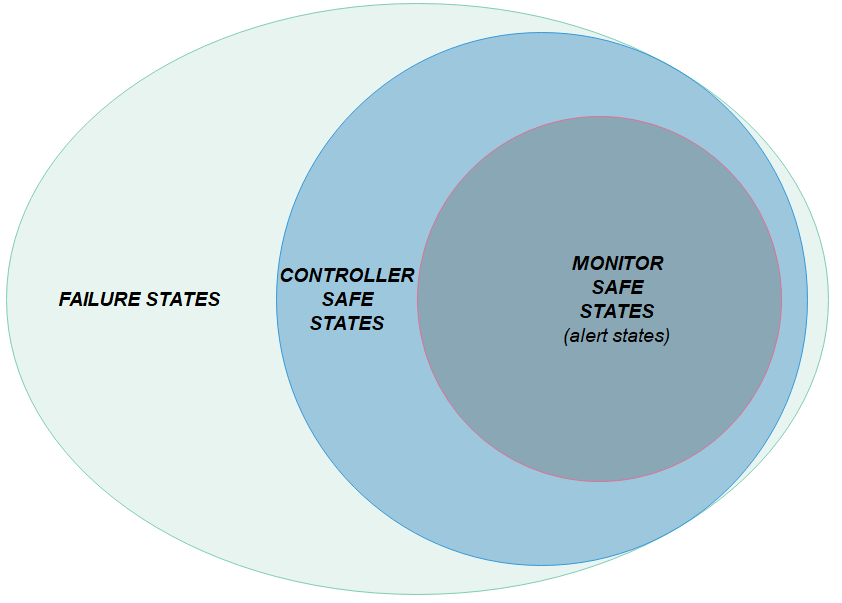
\includegraphics[width=\textwidth]{img/area-growth-bad.png}
	\captionof{figure}{The Controller now covers all the states previously covered by the Monitor, but doesn't cover anymore some of the states he covered before the training}
\end{minipage}

\chapter{System Analysis Method}

The goal of this work is to develop and to assess the feasability of an experimental method that allows to study the interaction between the AI controller and the Safety Monitor, with particulare attention to these aspectes:

\begin{itemize}
	\item How much and in what way the benefits given from the use of a safety-monitor can vary the more the neural network learns
	\item How much vary the effectiveness of the same monitor when applied to two different networks
	\item What features of the monitor determines an improvement (or worsening) to the safety of the system
	\item What aspects of the neural network training have an impact on the monitor usefulness
\end{itemize}

Safety-Monitors are developed in order to detect failures undetected by the network, therefore it is desiderable that the failures covered by the monitor don't overlap with the failures detected by the network. If this will be almost certainly true when the network is in the early stage of training, the lack of scientific results in this topic raises some concerns, while in the industry the long-time usefulness of the safety monitor is not even questioned.\newline
The problem when it comes to neural network is that, since they learn in a way that humans can loosely control, we can't predict what will be the most likely safety-hazard scenarios, nor we can efficiently test them. [assessing ultra-high dependability]

The reasoning behind this study is that it can not be guaranteed the long-time usefulness of the safety-monitor [assessing asymmetric systems EQ. 11].\newline

coverage dei casi coperti dal monitor come cambia

\section{Tools and softwares}

\subsection{Carla Simulator}

In order to have a realistic environment, with accurate physics simulation and data sensors, the open-source simulator Carla was used. This simulator was developed with the purpose of offering an environment where AI agents can be trained to drive.\newline

\begin{itemize}
	\item CARLA
	\item Nervana Systems - coach (Intel)
	\item Reti neurali su git
	\item Point Cloud Library per filtrare i dati
\end{itemize}

\section{Architettura del software (estrapolazione dati, interazione rete-monitor)}

\begin{itemize}
	
	\item Interazione rete-monitor
	\item Safety Monitor Implementation - obstacle detection
	\item Come vengono raccolti i dati
	\item Come vengono preprocessati
	
\end{itemize}

\section{Experiments methodology}

The study consists of several experiments in which we observe how the coverage of the safety-monitor (i.e. the probability of raising an alert if there really is a safety-hazard) vary with respect to a neural network in different stages of training.\newline
The first step to perform the analysis is to define what are the metrics of interest and how these can be measured. This task is harder than it seems because it's unknown \textsl{a priori} what the probability distribution function of the hazardous scenarios will be. This means that we don't know whether the probability of observing a failure depends on the \textsl{running time} of the experiment (e.g. the more the agent drives, the more likely a failure will happen) or if it depends on other factors.\newline
For this reason we decided to measure the length of an experiment in terms of number of failures: given the same initial scenario, two agents (one communicating with the monitor, the other relying solely on the AI) are let driving until n failures happen. We then observe the elapsed time between the start of the experiment and the moment the n^{th} failure happened.\newline
(Other metrics: velocita` a cui andava la macchina), (direzione da cui veniva l'altro veicolo se incidente)
---> per capire le situazioni in cui sbaglia di piu`

	\begin{itemize}
		
		\item Come vengono effettuati gli esperimenti (scenari? durata fissa? ad oltranza? fino ad un fallimento? \dots)
		\item Misure scelte - estrapolazione misure
		
	\end{itemize}

\chapter{Risultati dell'analisi}

In questa sezione elenchiamo i dati che sono stati raccolti e quali sono i risultati che abbiamo ottenuto (errori ricorrenti, grafici, rapporto monitor-rete neurale)
\chapter{Conclusions}

In this work we explored the topic of how to perform a monitoring activity on self-driving cars, controlled by a Control System (Controller) and a System Supervisor (Safety-Monitor).

This study is meant to be a first step on the analysis of \textsl{how a monitoring activity should be performed for such systems}, as they require particular care due to their complexity, and the critical issues of the environment in which they operate. Autonomous Vehicles themselves are not a new kind of systems, since they are commonly employed in military actions. However, the fact that self-driving cars will work at close contact with people and that the urban environment requires extra care in handling the moltitude of events (hazardous or not) that may happen.
Moreover, we questioned if there are relationships between the effectiveness of the Safety-Monitor component and the Controller component, when the latter gets trained for long periods, using different strategies.

In the first sections, we reviewed the main concepts of these activities, such as

\begin{itemize}
	\item The definition of \textsl{dependability} and \textsl{safety}, which are central to Safety-Critical Systems, are seen in the light of self-driving cars
	\item The problems that prevent us to deploy self-driving cars in urban environments at this level of knowledge
	\item How a wrong/poor/optimistic \textsl{dependability assessment} of these systems may have tragic consequences when these systems are deployed
	\item The problems of studying the observed emergent behaviour resulting from the interaction of two main Constituent Systems
	\item If, and in what way, the Safety-Monitor effectiveness is influenced by the performances of the Controller, in terms of:
	\begin{itemize}
		\item[-] Length of the training period
		\item[-] Strategies adopted during the training
	\end{itemize}
\end{itemize}

The development of this first methodology has taken into account the tools available for this kind of activities. Since most technologies in this field are private and proprietary, we had to look for open-source equivalents, demonstrating that it's not easy to perform these analyses in non-professional environments.

CARLA is with no doubt the best self-driving car simulator available, but it's not perfect. The LiDAR sensor bug\cite{lidarbug} would have prevented us to do this study and if it wasn't for the project developed by Zhuang\cite{carlapro}, it would have been \textsl{unfeasable} because our only alternative would have been to use \textsl{ground-truth} data, which would have been pointless for this work.

If on one hand, \textsl{Coach framework} is developed by \textsl{Intel AI Labs}, it suffers from the common issues often found in open-source project, the most evident being one of the two agents provided for CARLA, which stopped moving after few stages of training in \textsl{phase 1} (therefore unrelated to the use of Safety-Monitor).
This bug makes us wonder about the presence of other issues in the design of the training algorithm which may had an influence on the behaviours observed for $C5_{S2\dots 4}$.

Another issue that mines the usability of this framework is that the RAM is not correctly freed, eventually filling it and causing a crash of the running processes. This required us to monitor the training execution and restart it at every crash.\newline

The monitoring activity was developed keeping in mind the main properties of:

\begin{itemize}
	\item Repeatibility
	\begin{itemize}
		\item[-] By recording the Controller's execution in files, saving the action taken by the Controller in each frame and the seeds used in RNGs\footnote{Random Number Generators}, the Destination Goals and the environmental parameter of each scenario
	\end{itemize}
	\item Non-Intrusiveness
	\begin{itemize}
		\item[-] Code instrumentation, as said, may produce non-real time data or wrong measurements, due to the client-server architecture used. CARLA solves this problem by allowing users to run simulations at a \textsl{fixed time step}. However the hardware must be powerful enough to achieve the time step required
	\end{itemize}
	\item Representativeness
	\begin{itemize}
		\item[-] Representativeness of \textsl{test-cases} is one of the central problems when monitoring self-driving cars, because hazardous events may be so complex and so many that is impossible to consider them all. The definition of scenarios and difficulty level helps in this sense, providing many different sitations starting from the same scenario
		\item[-] Representativeness of the \textsl{measures} computed for the Safety-Monitor raised issues on the nature of the dataset we are working with. The choice of the measures to be used on the Confusion Matrix was explained and motivated, as well as the exclusion of the others
	\end{itemize}
	\item Feasibility
	\begin{itemize}
		\item[-] The research on the best tools to be used for this activity was not easy, due to the multitude of solutions proposed that in reality have lots of practical limitations. However, the tools used in this work allowed us to perform this activity. At the same time we can not ignore the issues found in these projects
	\end{itemize}

\end{itemize}

If the \textsl{feasibility} property is undermined by the presence of issues in the tools used, the methodology developed still proved to be an effective way of assessing the reliability of Autonomous Vehicles allowing us to approximate all the common measures of interest for these systems, without sticking to common metrics used in the evaluation of neural networks, e.g. the \textsl{Loss Function}, which indeed are powerful and mandatory measures to compute to check that the neural network is actually learning, but doesn't give any evidence at all on the goodness of the System in its entirety.

This methodology proved to be an effective mean to study the behaviour of the whole System, focusing on well-known measures used to assess a system's dependability and the Safety-Monitor's performances. The definition of \textsl{Scenarios} and \textsl{difficulties} is very useful in the understanding of what environmental parameters cause a degradation on System's performances and in the generation and analysis of \textsl{"uncommon"} situations that not always can be taken into account when designing \textsl{ad-hoc safety-cases}
\newline

The main conjecture that made us start this work, was if "static" (in the sense that they don't learn from new data) error-checkers' performances were depending on the performances of neural networks and if ad hoc training strategies have an influence as well. From the data collected it looks like the Monitor's effectiveness is likely to change with expert agents, motivating us to continue to study in deep this conjecture.

The failure of those strategies that used the Safety-Monitor to guide the training ($S2,\: S3,\: S4$) did not give us evidences on this fact, and this problem was already discussed in the previous chapter. This failure may be caused by two factors:

\begin{itemize}
	\item[1)] Misspecified reward function
	\item[2)] The training period was not long enough
\end{itemize}

The fact that the agents trained were not getting unintentionally high reward for standing still, makes us think that the neural network needed more time to learn what the Safety-Monitor is trying to teach. A higher \textsl{simulation time step} could have helped us, making \textsl{simulation time} running faster than \textsl{real time}. However, this required ultra-high performance hardware, therefore we could not train the models for more time, nor retrain the networks adjusting the reward parameters.

At the same time, the Safety-Monitor proved to be \textsl{less} effective when operating in combination with the Checkpoint which had the \textsl{best} performances and, most of all, it was the one obtained from Checkpoint $C4$ by changing the training strategy, while when operating with the Checkpoints trained with strategy $S0$ $(C1,\: C2,\: C3,\: C4,\: C5_{S0})$ it had the same TPR ($0.75$), with the exception of $C2$. If on one hand, $C2$ was definetely a special case, for the reasons listed in the previous chapter, at the same time we can not exclude the same hypothesis for $C5_{S1}$. In future works, we want to continue the training of $C5_{S1}$ to confirm this fact.\newline

This work demonstrated the power of the use of a simulated environment for the assessment self-driving cars, taking into account and solving many of the problems found when approximating the measures of interest for these systems, and common problems found in a monitoring activity.

In future works, our interest will be:

\begin{itemize}
	\item Developing stochastical models based on data collected with this monitoring methodology, to guide us in the tunning of the reward function parameters
	\item Continuing the training of $C5_{S0\dots 4}$ to:
	\begin{itemize}
		\item[a)] Collect more evidences about the effectiveness of the Safety-Monitor
		\item[b)] Have a better understanding of the failure causes of strategies $S2\dots 4$
	\end{itemize}
	\item Applying the same monitoring methodology using more powerful tools (e.g. proprietary software, pretrained neural networks, better Safety-Monitor)
\end{itemize}

\begin{thebibliography}{9}

\bibitem{striginiPopov}
Peter Popov, Lorenzo Strigini - \textit{Assessing Asymmetric fault-tolerant Software}

\bibitem{randstudy}
Nidhi Kalra, Susan M. Paddock - \textit{Driving to Safety: How Many Miles of Driving Would It Take to Demonstrate Autonomous Vehicle Reliability?}

\bibitem{arizuber}
Arizona 2018 Uber Incident - \textit{https://en.wikipedia.org/wiki/Death\_of\_Elaine\_Herzberg}

\bibitem{elonmusk}
Elon Musk declarations - \textit{https://techcrunch.com/2020/02/18/elon-musk-says-all-advanced-ai-development-should-be-regulated-including-at-tesla}

\bibitem{govarizuber}
Uber incident Preliminary Report - \textit{https://www.ntsb.gov/investigations/AccidentReports/Reports/HWY18MH010-prelim.pdf}

\bibitem{koopman}
Philip Koopman - \textit{http://safeautonomy.blogspot.com/}

\bibitem{carla}
CARLA - \textit{http://carla.org/}

\bibitem{lidarbug}
CARLA LiDAR Bug - \textsl{https://github.com/carla-simulator/carla/issues/1212}


\bibitem{carlapro}
Improved LiDAR CARLA - \textsl{https://github.com/ZhuangYanDLUT/carla}

\bibitem{coach}
Nervana Systems - Coach - \textit{https://github.com/NervanaSystems/coach}

\bibitem{zhaoStrigini}
Xingyu Zhao, Valentin Robu, David Flynn, Kizito Salako, Lorenzo Strigini - \textit{Assessing the Safety and Reliability of Autonomous Vehicles from Road Testing}

\bibitem{littlewoodStrigini}
Bev Littlewood, Lorenzo Strigini - \textit{Validation of Ultra-High Dependability for Software-based Systems}

\bibitem{retinaNet}
Tsung-Yi Lin, Priya Goyal, Ross Girshick, Kaiming He, Piotr Dollár - \textit{Focal Loss for Dense Object Detection}

\bibitem{alphaGo}
DeepMind - \text{https://deepmind.com/research/case-studies/alphago-the-story-so-far}

\bibitem{alphaGoBeatsMan}
Google AI defeats human Go champion - \textit{https://www.bbc.co.uk/news/technology-40042581}

\bibitem{foolnn}
Anh Nguyen, Jason Yosinski, Jeff Clune - \textit{Deep Neural Networks are Easily Fooled: High Confidence Predictions for Unrecognizable Images}

\bibitem{stupidnn}
Christian Szegedy, Wojciech Zaremba, Ilya Sutskever, Joan Bruna, Dumitru Erhan, Ian Goodfellow, Rob Fergus - \textit{Intriguing properties of neural networks}

\bibitem{coachIssue}
Coach Issue - \textit{https://github.com/NervanaSystems/coach/issues/428}

\bibitem{ddpg}
Timothy P. Lillicrap, Jonathan J. Hunt, Alexander Pritzel, Nicolas Heess, Tom Erez, Yuval Tassa, David Silver, Daan Wierstra - \textit{Continuous control with deep reinforcement learning}

\bibitem{pointcloud}
Point Cloud Format - \textit{https://en.wikipedia.org/wiki/Point\_cloud}

\bibitem{pclwiki}
Point Cloud Library Info - \textit{https://en.wikipedia.org/wiki/Point\_Cloud\_Library}

\bibitem{pcl}
Point Cloud Library - \textit{http://pointclouds.org/}

\bibitem{rss}
Responsibility-Sensitive Safety - \textit{https://www.mobileye.com/responsibility-sensitive-safety/}

\bibitem{dependabilitypaper}
J.C. Laprie - \textsl{Dependability - its attributes impairments and means, Predictability Dependable Computing Systems}

\bibitem{safety-critical}
J.C. Knight - \textsl{Safety Critical Systems: Challenges and Directions, Proceedings of the 24th International Conference on Software Engineering}

\bibitem{bonda}
Andrea Bondavalli - \textsl{L'analisi quantitativa dei Sistemi Critici, Fondamenti e Tecniche per la Valutazione - Analitica e Sperimentale - di Infrastrutture Critiche e Sistemi Affidabili}

\bibitem{monitor1}
G.J. Nutt - \textsl{Tutorial: Computer system monitors}

\bibitem{monitor2}
B. Plattner - \textsl{Real-time execution monitoring}

\bibitem{monitor3}
B.Plattner, J. Nievergelt - \textsl{Special feature: Monitoring program execution: A survey}

\bibitem{LOD}
Engin Bozkurt - \textsl{https://github.com/enginBozkurt/LidarObstacleDetection}

\bibitem{reward1}
Erik Talvitie - \textsl{Learning the Reward Function for a Misspecified Model}

\bibitem{reward2}
Ellis Ratner, Dylan Hadfield-Menell, Anca D. Dragan - \textsl{Simplifying Reward Design	through Divide-and-Conquer}

\bibitem{reward3}
Nicolas Heess, Greg Wayne, David Silver, Timothy Lillicrap, Yuval Tassa, Tom Erez - \textsl{Learning Continuous Control Policies by Stochastic Value Gradients}

\bibitem{rewardtrialanderror1}
Yingjun Ye, Xiaohui Zhang, Jian Sun - \textsl{Automated Vehicle's behavior decision making using deep reinforcement learning and high-fidelity simulation environment}

\bibitem{rewardtrialanderror2}
Sampo Kuutti, Saber Fallah, Richard Bowden, Phil Barber - \textsl{Deep Learning for Autonomous Vehicle Control - Algorithms, State-of-the-Art, and Future Prospects}

\bibitem{wikiconfmatrix}
Confusion Matrix, Wikipedia - \textsl{https://en.wikipedia.org/wiki/Confusion\_matrix}

\bibitem{isoacc}
ISO 5725-1:1994 - \textsl{Accuracy (trueness and precision) of measurement methods and results}

\bibitem{mcc}
Davide Chicco, Giuseppe Jurman - \textsl{The advantages of the Matthews correlation coefficient (MCC) over F1 score and accuracy in binary classification evaluation}


\end{thebibliography}




%--------------------------------------------------------------
\end{document}
%--------------------------------------------------------------